% Template for ICASSP-2017 paper; to be used with:
%          spconf.sty  - ICASSP/ICIP LaTeX style file, and
%          IEEEbib.bst - IEEE bibliography style file.
% --------------------------------------------------------------------------
\documentclass{article}
\usepackage{spconf,amsmath,graphicx}
\usepackage{bm}
\usepackage{hyperref}
\usepackage{url}
\usepackage{amsmath}
\usepackage{amsthm}
\usepackage{amsfonts}
\usepackage{graphicx}
\usepackage{subcaption}
\usepackage{hyperref}
\usepackage{algorithm2e}
\usepackage{pbox}
\usepackage{multirow}

% Example definitions.
% --------------------
\def\x{{\mathbf x}}
\def\L{{\cal L}}

% Title.
% ------
\title{INVARIANT REPRESENTATIONS FOR NOISY SPEECH RECOGNITION}
%
% Single address.
% ---------------
%\name{Dmitriy Serdyuk $^{\dagger}$ \qquad Kartik Audhkhasi$^{\star}$ \and Philemon Brakel$^{\dagger}$ \and Bhuvana Ramabhadran$^{\star}$  \and Yoshua Bengio$^{\dagger}$\thanks{Yoshua Bengio is a CIFAR Fellow.}}
%\address{$^{\dagger}$ Universit\'e de Montr\'eal, $^{\star}$ IBM}
%
% For example:
% ------------
%\address{School\\
%	Department\\
%	Address}
%
% Two addresses (uncomment and modify for two-address case).
% ----------------------------------------------------------
\twoauthors
  {Dmitriy Serdyuk $^{\dagger}$\thanks{Dmitriy Serdyuk performed the work
  while at IBM}, Kartik Audhkhasi$^{\star}$, Phil\'emon Brakel$^{\dagger}$, Bhuvana Ramabhadran$^{\star}$, Yoshua Bengio$^{\dagger}$\thanks{Yoshua Bengio is a CIFAR Fellow.}}
  {$^{\dagger}$ Universit\'e de Montr\'eal \\
  $^{\star}$ IBM}
  {}
  {}


\begin{document}
%\ninept
%
\maketitle
%
\begin{abstract}
    Robustness of a speech recognition system is a challenging task and modern
    automatic speech recognition (ASR) systems need to be resilient to different recording conditions,
    microphone type, accents, and noisy recording environment. We mitigate
    this problem in a fashion similar to recent research on image generation using
    Generative Adversarial Networks and domain adaptation ideas extending
    adversarial gradient-based training. A recent work of Ganin et al. proposes to
    use adversarial training procedure for image domain adaptation making an intermediate
    representation to improve the target performance and at the same time
    to deteriorate the domain classifier performance, which is a separate neural
    network taking the intermediate representation as the input.

    This work focuses on investigation of neural architectures which produce
    representations invariant to certain conditions as the noise type for speech
    recognition. Similar
    to the Ganin et al. work we train the intermediate representation to be invariant
    to noise conditions training three neural networks: the encoder, the recognizer, and the
    noise classifier to produce the representation produced by the encoder to decrease
    the performance of the classifier making the representation invariant to noise conditions. We
    experimentally evaluate proposed architectures on the acoustic modelling task
    for speech recognition on a popular benchmark Aurora4.
\end{abstract}
%
\begin{keywords}
speech recognition, deep neural networks, invariant representations, adversarial training
\end{keywords}
%
\section{Introduction}
\label{sec:intro}
    One of the most challenging aspects of automatic speech recognition (ASR),
    is the mismatch between the training and testing conditions. During
    testing, a system may encounter new recording conditions, microphone types,
    accents and types of background noises. Even if all testing conditions also appeared
    in the train data, their relative distribution is likely to be
    different. For this reason, it's important to develop systems that are
    robust towards changes in recording conditions in general.

    While many types of model and feature based adaptation methods like MLLR and fMLLR
    \cite{leggetter1995maximum} have been proposed, most of these methods have
    been designed with GMM-HMM systems in mind. Since the enormous success of
    Deep Neural Network (DNN) systems for ASR \cite{hinton2012deep}, GMM-based
    model adaptation is not possible anymore, while feature-based methods may
    not be optimal anymore.
    Moreover, the discriminative gradient-based optimization used to train
    DNNs, in combination with the ability of DNNs to learn highly non-linear
    feature transformations, allows for more flexibility when it comes to the
    construction of training objectives that promote domain invariant
    representations.

    The main idea of this work is that instead of training a robust system,
    it is possible to train a system which will be invariant to these 
    conditions. This method of training requires the labels in the dataset
    which indicate which condition a particular recording was taken in, the 
    test data doesn't need to contain these labels. The method was proposed in
    the context of image classification in~\cite{ganin2014unsupervised} and 
    will be explained in Section~\ref{sec:gradient-reverse} and the application 
    to speech recognition is discussed
    in Section~\ref{sec:invariant-speech}. It is tightly connected to the idea
    of generative adversarial networks (GAN) proposed 
    in~\cite{goodfellow2014generative} thus we start with the discussion
    on this type of generative networks in Section~\ref{sec:gans}

    %TODO

\section{Generative Adversarial Networks}
\label{sec:gans}
    One of the most insightful recent advantages in the area of generative models
    is the models of the family of generative adversarial networks (GAN).
    A GAN consists of two networks: generator and discriminator. The generator 
    network $G$ has an
    input of randomly generated vector and is asked to produce an image 
    similar to the images in the training set. The discriminator network $D$
    can either receive a generated image from the generator $G$ or an image
    from the training set, the task of the discriminator is to distinguish
    between a generated image and a ``real'' image taken from the dataset. Thus
    the discriminator is just a classifier network with a sigmoid output
    and can be trained with the gradient methods (see 
    Section~\ref{sec:optimization}). The main idea of the generative adversarial
    training is that it is possible to propagate the gradient of the discriminator
    network further to the generator network staking them on top of each other.
    This leads to an efficient training procedure and GANs achieve the state of the
    art that time on handwritten digit generation MNIST dataset.

    In other words, these two networks are competing with each other the 
    generator is trying to deceive the discriminator network while it tries
    to do its best to recognize if there was a deception. This game theoretical
    similarity gave a name of adversarial networks. The objective of adversarial
    training is following
    \begin{align*}
        \min_G \max_D V(D, G) = \mathbb{E}_{\bm{x} \sim p_{\text{data}}(\bm{x})}[\log D(\bm{x})] + \\
          \mathbb{E}_{\bm{z} \sim p_{\bm{z}}(\bm{z})}[\log (1 - D(G(\bm{z})))].
    \end{align*}

    One of the properties of GAN networks that there is no straightforward way 
    to evaluate the quality of image generation process since the GAN doesn't 
    output the log-likelihood of its samples. The paper estimated the likelihood
    using the Parzen windows estimator.

    In practice, GANs might be hard to train due to the fact that in a case when 
    the discriminator is more powerful that the generator, the later doesn't 
    receive any gradient thus can not be improved. Usually this problem is solved
    using a smart schedule which stops learning the discriminator as soon as it
    is too far ahead of the generator. Other possible solutions include ``soft''
    targets bounded at some constant rather than between 0 and 1 and using a 
    different proxy for the cost.

\section{Gradient Reverse Method}
\label{sec:gradient-reverse}

    A work~\cite{ganin2014unsupervised} proposes a method of training a network 
    which can be adapted to new domains. The training set consists of the images
    labeled with classes and the separate domain labels. The test set doesn't need
    to have the domain labels. For example, it may be first domain
    consisting of MNIST digits and second domain of MNIST digits on a different
    background. The network has a fork-like structure: the image is fed to the
    first network which produces a hidden representation $h$, then there are two
    networks branching of the representation $h$: a domain classifier network and 
    a target classifier. The goal of the training is to produce the hidden 
    representation invariant to the domain labels so that information doesn't 
    interfere the target classifier which is used in the test time.

    The network is trained with three goals: the hidden representation $h$ should
    be helpful for the target classifier, but harmful for the domain classifier,
    the domain classifier should have a good classification accuracy. More 
    formally, we define the objective as
    \begin{equation}
        L = L(\hat{y}, y; \theta_R, \theta_C) + 
        \alpha L(\hat{d}, d; \theta_D) -
        \beta L(\hat{d}, d; \theta_R),
    \end{equation}
    where $y$ is the ground truth class, $d$ is the domain label, corresponding
    hatted variables are the network predictions, $\theta$ are the network 
    parameters, and $R, C, D$ are the subsets of parameters in the representation,
    classifier and domain adaptation networks respectively. The hyper-parameters
    $\alpha$ and $\beta$ denote the influence of every part of the cost.

\section{Related Work}

\section{Experiments}
We experimentally evaluate the approach discussed in Section~\ref{sec:gradient-reverse} 
on a noisy speech recognition dataset Aurora-4~\cite{parihar2002aurora}. This dataset
is based on the Wall Street Journal (WSJ0 is available at LDC). Additive noise of 
six categories (airport, babble, car, restaurant, street, train) was introduced to the 
clean data. We used mel-filterbank features with their deltas and delta-deltas spliced
over 5 frames on each side making 11 consecutive frames and 1320 input features. 
We did not use any speaker normalization of input features. We pretrained 5 layer
speech recognition network with 2048 rectified linear units at every layer using Adam 
optimization algorithm for 5 epochs. After pretraining, we turned on the invariance term.

First expriment we performed is the gender invariance. We added a 2 layer network 
branching off the last layer of the pretrained speech recognition network and 
trained it until convergence with SGD. Although, the performance remained unchanged,
the t-SNE visualization on Figure~\ref{fig:tsne} demonstrates that the hidden units
are less separated in the projected space.

\begin{figure}
    \centering
    %TODO: add image
    \begin{subfigure}[b]{0.5\linewidth}
        \centering
        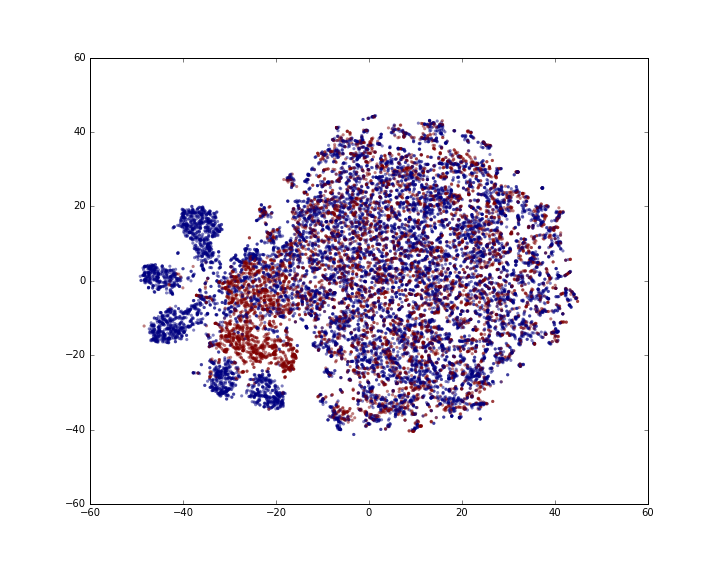
\includegraphics[width=\linewidth]{tsne-original.png}
    \end{subfigure}%
    \begin{subfigure}[b]{0.5\linewidth}
        \centering
        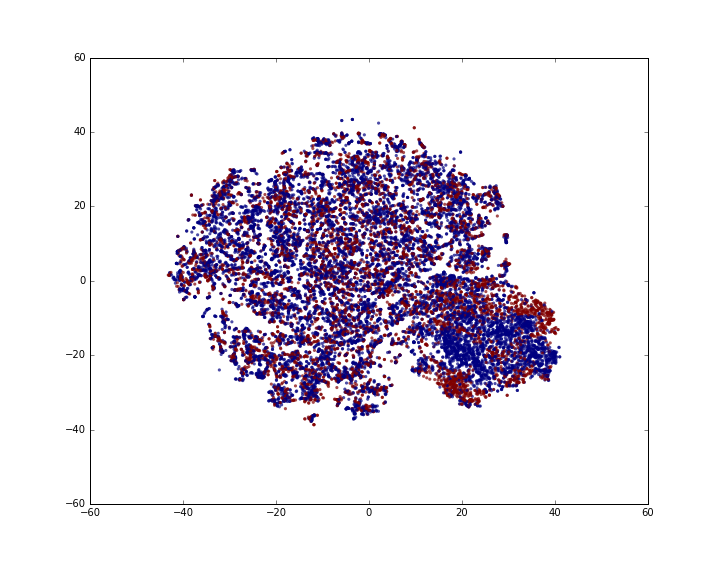
\includegraphics[width=\linewidth]{tsne-invariant.png}
    \end{subfigure}%
    \caption{t-SNE visualization of the last hidden layer. On the left, the baseline
    model. On the right, the model trained with the adversarial objective. Colors 
    represent genders.}
    \label{fig:tsne}
\end{figure}

\section{Conclusion}


\section*{Acknowledgments}

We would like to thank Yaroslav Ganin, David Warde-Farley for insightful discussions,
developers of Theano~\cite{2016arXiv160502688short}, Blocks, and Fuel~\cite{MerrienboerBDSW15} 
for great instruments.

% References should be produced using the bibtex program from suitable
% BiBTeX files (here: strings, refs, manuals). The IEEEbib.bst bibliography
% style file from IEEE produces unsorted bibliography list.
% -------------------------------------------------------------------------
\bibliographystyle{IEEE}
\bibliography{refs}

\end{document}
